\documentclass[fleqn]{NotesClass}

\usepackage{siunitx}
\usepackage{csquotes}
\usepackage{subcaption}

% Tikz stuff
\usepackage{tikz}
\tikzset{>=latex}
% external
\usetikzlibrary{external}
\tikzexternalize[prefix=tikz-external/]
%\tikzexternaldisable
% other libraries
\usetikzlibrary{hobby}

% References, should be last things loaded
\usepackage{hyperref}  % Should be loaded second last (cleveref last)
\colorlet{hyperrefcolor}{blue!60!black}
\hypersetup{colorlinks=true, linkcolor=hyperrefcolor, urlcolor=hyperrefcolor}
\usepackage[
capitalize,
nameinlink,
noabbrev
]{cleveref} % Should be loaded last

% My packages
\usepackage{mathtools}
\usepackage{NotesBoxes}
\usepackage{NotesMaths}

% Title page info
\title{Statistical Physics}
\author{Willoughby Seago}
\date{}
% \subtitle{}
% \subsubtitle{}

% Highlight colour
\definecolor{highlight}{HTML}{00FF22}
\definecolor{my blue}{HTML}{00AAFF}
\definecolor{my red}{HTML}{FF2200}
\definecolor{my yellow}{HTML}{FFEE00}
\definecolor{my purple}{HTML}{CC00FF}

% Commands
% Maths
\newcommand*{\indicator}{\mathbf{1}}
\newcommand*{\order}{\mathcal{O}}
\newcommand*{\e}{\mathrm{e}}
\newcommand*{\boltzmann}{k_{\mathrm{B}}}

% Include
\includeonly{}

\begin{document}
    \frontmatter
    \titlepage
    \innertitlepage{tikz-external/the-ising-model.pdf}
    \tableofcontents
    \mainmatter
    
    \part{Monte Carlo and the Ising Model}
    \chapter{Monte Carlo}
    \defineindex{Monte Carlo} algorithms, named after the Monte Carlo casino, are stochastic methods for computing integrals.
    In a Monte Carlo computation we approximate the value of an integral by a series of averages.
    
    \section{Averages}
    Given a random variable, \(x_i\), the average is defined as
    \begin{equation}
        \expected{x} \coloneqq \frac{1}{n} \sum_{i=1}^{n} x_i
    \end{equation}
    where the sum is over all measurements of \(x\).
    Similarly if \(f\) is a function of the random variable \(x_i\) then the average value of this function is
    \begin{equation}
        \expected{f(x)} \coloneqq \frac{1}{n} \sum_{i=1}^{n} x_if(x_i) = \sum_{i=1}^{n} x_if_i
    \end{equation}
    where we define \(f_i = f(x_i)\).
    
    Often we instead want to work with weighted averages, say if certain outcomes are more likely than others.
    If outcome \(i\) has weight \(w_i\) then the weighted average of the random variable \(x_i\) is
    \begin{equation}
        \expected{x} \coloneqq \frac{\sum_{i=1}^{n} x_iw_i}{\sum_{i=1}^{n} w_i}.
    \end{equation}
    The weighted average of \(f\) is similarly
    \begin{equation}
        \expected{f(x)} \coloneqq \frac{\sum_{i=1}^{n} f(x_i)w_i}{\sum_{i=1}^{n}w_i}.
    \end{equation}
    
    \section{Monte Carlo Integration}
    Suppose we wish to compute the \(d\)-dimensional integral
    \begin{equation}
        I = \int_V f(\vv{r}) \dd{^dr}.
    \end{equation}
    First note that we can write this as an integral over all space by writing it as
    \begin{equation}
        I = \int_{\reals^d} f(\vv{r}) \indicator_V(\vv{r}) \dd{^dr}
    \end{equation}
    where \(\indicator_V\) is the indicator function for \(V\), defined by \(\indicator_V(\vv{r}) = 1\) if \(\vv{r} \in V\) and \(\indicator_V(\vv{r}) = 0\) if \(\vv{r} \notin V\).
    
    Using the fact that
    \begin{equation}
        V = \int_V \dl{^dr}
    \end{equation}
    is the volume of the integration region we can write the integral as
    \begin{equation}
        I = \frac{\int_V f(\vv{r}) \dl{^dr}}{\int_V \dl{^dr}} V.
    \end{equation}
    Notice now the similarity to the weighted average with all weights being 1, which is just the normal average, simply change integrals to sums.
    We therefore have
    \begin{equation}
        I = \frac{\int_V f(\vv{r}) \dd{^dr}}{\int_V \dl{^dr}} V \approx \frac{\sum_{i} f(\vv{r_i})}{\sum_i 1} = \expected{f(\vv{r})}.
    \end{equation}
    
    The process of calculating an integral becomes the process of computing an average.
    
    If we take \(n\) samples then the sum in the denominator is simply \(n\) and we have
    \begin{equation}
        I \approx \frac{\sum_{i=1}^{n} f_i}{n}V.
    \end{equation}
    This is our Monte Carlo estimate of the integral.
    
    The error on this measurement is associated with the standard error on the mean, since we are calculating a sample mean but really we want the population mean, that is \(n \to \infty\).
    The standard error on the mean is
    \begin{equation}
        \frac{\sigma}{\sqrt{n}} \sim n^{-1/2}
    \end{equation}
    where \(\sigma\) is the standard deviation.
    We clearly want \(n\) to be large in order to have a small error.
    
    \subsection{Trapezium Rule}
    An alternative method for approximating integrals is to split the integration region into sections, we then approximate \(f\) as linear over these sections.
    Define \(\overline{f_i}\) to be the average value of this linear approximation of \(f\) in the \(i\)th section.
    The integral is then approximated as the total volume of these sections that we have split the integral into.
    That is
    \begin{equation}
        I = \int_V f(\vv{r}) \dd{^d r} \approx \sum_i \text{volume of \(i\)th trapezium} = \sum_i \delta^d \overline{f_i}
    \end{equation}
    where \(\delta^d\) is the area of the base of the section, assuming we split the space evenly into a grid spaced \(\delta\) apart, and \(\overline{f_i}\) is the average height of the linear approximation of the function in this region.
    For a one-dimensional integral these small sections are trapeziums, hence the name trapezium rule.
    
    The error in our approximation of the function is \(\order(\delta^2)\) since we have approximated \(f\) as linear.
    The error then scales as \(n \delta^d \delta^2\) where \(n\) is the number of regions.
    The number of regions is the integration volume divided by the volume of each region, \(n = V/\delta^d\), and so \(\delta^d \sim 1/n\), which means \(\delta \sim n^{-1/d}\).
    The error therefore scales as \(nn^{-1}n^{-2/d} = n^{-2/d}\).
    
    Comparing this to the error for the Monte Carlo method we see that if \(d > 4\) the error on the Monte Carlo method actually decreases faster than the error for the more complex trapezium rule.
    
    \section{Statistical Physics}
    In statistical physics the Monte Carlo method can be used to compute thermodynamic averages.
    A system with a fixed number of particles, \(N\), is a canonical ensemble and the physics is dictated in part by the partition function
    \begin{equation}
        Z \coloneqq \sum_{\mathclap{i \in \{\text{states}\}}} \e^{-\beta E_i}
    \end{equation}
    where \(\beta \coloneqq 1/(\boltzmann T)\) with \(E_i\) being the energy of state \(i\), \(\boltzmann\) being Boltzmann's constant and \(T\) the temperature.
    
    The average of some observable, \(A\), is then given by summing over all states, \(i\):
    \begin{equation}
        \expected{A} \coloneqq \frac{\displaystyle\sum_{i} A_i\e^{-\beta E_i}}{\sum_{i} \e^{-\beta E_i}} = \frac{1}{Z} \sum_{i} A_i\e^{-\beta E_i}.
    \end{equation}
    That is \(\expected{A}\) is the weighted average with weight \(w_i = \e^{-\beta E_i}\).
    
    Writing this same value as
    \begin{equation}
        \expected{A} \approx \frac{\sum_{i=1}^{n} A_i\e^{-\beta E_i}}{n} \frac{n}{\sum_{i=1}^{n} \e^{-\beta E_i}},
    \end{equation}
    here we've introduced a factor of \(n/n = 1\), as well as approximating the sums over all states with sums over \(n\) states.
    Notice that the first term is the Monte Carlo estimate of the average of \(A\) and the second is the reciprocal of the Monte Carlo estimation of the partition function.
    
    The question is how we sample the states.
    The obvious answer of uniformly sampling the states turns out not to work, as we will see in the next section.
    
    \section{The Ising Model}
    The Ising model is a simple model that can be used to demonstrate several concepts in statistical mechanics.
    The \defineindex{Ising model} consists of a lattice of equally spaced points and we imagine that at each point there is a particle which can have either spin up or spin down.
    We will work with a two-dimensional grid.
    We index the points from \(1\) to \(N\), although we could also index each point by its row an column, which is often more useful in code.
    To each point \(i\) we assign a value of \(+1\) or \(-1\) depending on if the spin is up or down.
    We start with the spins chosen randomly and uniformly, so approximately half of the spins will be up and half down.
    
    \begin{figure}
        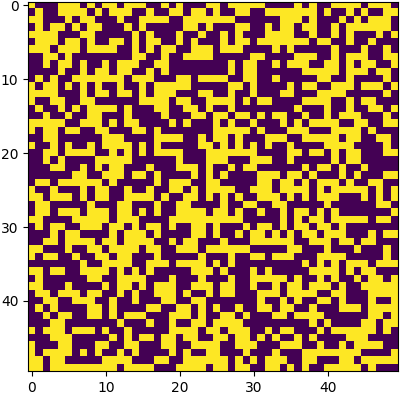
\includegraphics[height=0.3\textheight]{images/ising-random-start}
        \caption[Random Ising Model Start]{Initially the Ising model starts in a random state. Here opposite spins are represented by different colours. The axes are simply the row and column numbers, here \(50^2 = 2500\) sites has been used.}
    \end{figure}
    
    The energy of the system depends only on how the spins align.
    We assume the grid spacing is large enough that only interactions with the nearest neighbours have effect.
    The total energy of the system is then
    \begin{equation}
        E = -J\sum_{\langle i, j \rangle} S_iS_j
    \end{equation}
    where \(J\) is a positive constant with dimensions of energy and \(\langle i, j \rangle\) means that we sum over \(i\) and then \(j\) corresponds to the nearest neighbours.
    
    \begin{figure}
        \tikzsetnextfilename{the-ising-model}
        \begin{tikzpicture}
            \fill[use Hobby shortcut, closed, highlight!20] (-0.5, 1) .. (0, 0.5) .. (0.4, 0.4) .. (0.5, 0) .. (1, -0.5) .. (1.5, 0) .. (1.6, 0.4) .. (2, 0.5) .. (2.5, 1) .. (2, 1.5) .. (1.6, 1.6) .. (1.5, 2) .. (1, 2.5) .. (0.5, 2) .. (0.4, 1.6) .. (0, 1.5);
            
            \draw[<-] (0, -0.25) -- ++ (0, 0.5);
            \draw[<-] (1, -0.25) -- ++ (0, 0.5);
            \draw[<-] (2, -0.25) -- ++ (0, 0.5);
            \draw[<-] (0, 0.75) -- ++ (0, 0.5);
            \draw[->] (1, 0.75) -- ++ (0, 0.5);
            \draw[->] (2, 0.75) -- ++ (0, 0.5);
            \draw[->] (0, 1.75) -- ++ (0, 0.5);
            \draw[<-] (1, 1.75) -- ++ (0, 0.5);
            \draw[->] (2, 1.75) -- ++ (0, 0.5);
            
            \node [left, font=\ttfamily\footnotesize] at (0, 2) {1};
            \node [left, font=\ttfamily\footnotesize] at (1, 2) {2};
            \node [left, font=\ttfamily\footnotesize] at (2, 2) {3};
            \node [left, font=\ttfamily\footnotesize] at (0, 1) {4};
            \node [left, font=\ttfamily\footnotesize] at (1, 1) {5};
            \node [left, font=\ttfamily\footnotesize] at (2, 1) {6};
            \node [left, font=\ttfamily\footnotesize] at (0, 0) {7};
            \node [left, font=\ttfamily\footnotesize] at (1, 0) {8};
            \node [left, font=\ttfamily\footnotesize] at (2, 0) {9};
        \end{tikzpicture}
        \caption[The Ising model.]{A \(3 \times 3\) Ising model with spins represented by arrows. The shaded region is the nearest neighbours of spin 5, the central spin.}
        \label{fig:ising model}
    \end{figure}

    \Cref{fig:ising model} shows a \(3\times 3\) Ising model.
    The nearest neighbours of the \(5\)th point are points 2, 4, 6, and 8.
    The contribution to the sum when \(i = 5\) is
    \begin{equation}
        -J\sum_{\langle 5, j \rangle} S_5S_j = -JS_5(S_2 + S_4 + S_6  + S_8) = -J 1(-1 - 1 + 1 - 1) = 2 J
    \end{equation}
    Notice that if we flip spin 5, that is \(S_5 \to -S_5\), the change in energy is
    \begin{align}
        \Delta E &= -J(-S_5)(S_2 + S_4 + S_6  + S_8) - (-J)S_5(S_2 + S_4 + S_6  + S_8)\\
        &= 2JS_5(S_2 + S_4 + S_6  + S_8)\\
        &= 2J1(-1 - 1 + 1 - 1)\\
        &= -4J
    \end{align}
    This can be used to avoid having to calculate the energy of the entire model when we flip a single spin.
    
    In a general Ising model of \(N\) sites, which in our example is 9, there are 2 possible values of the spin at each site and hence there are \(2^N\) possible states.
    In our example there are \(2^9 = 512\) possible states.
    A more realistic size would be a \(50 \times 50\) grid which has \(N = 50^2 = 2500\), in which case \(2^{2500} \approx = 10^{752}\), which is huge.
    
    The physics of the model is determined entirely by \(\e^{-\beta E}\).
    Since \(E \propto J\) the only values that appear in the model, apart from the values of the spins, is the product \(\beta J = J/(\boltzmann T)\).
    We could use real values for these, for example \(J\) would be some factor of \(\hbar\) and \(\boltzmann \approx 10^{-23}\,\unit{\joule\per\kelvin}\).
    However, these incredibly small numbers would cause huge floating point errors.
    Instead it is better to use the fact that these parameters only ever appear in ratio, \(J/\boltzmann\), and so we could just use \(J/\boltzmann \approx 10^{-12} \, \unit{\second \kelvin}\).
    This is still tiny however and will lead to floating point issues.
    A better thing to do is to set \(J = \boltzmann = 1\), and then use \(T\) as the parameter measured in some units such that \(J = \boltzmann = 1\).
    
    It is energetically favourable for all of the spins to align, either all up or all down.
    This means that there are two states which are much more likely than all other states, in particular they are much more likely than disordered states.
    On the other hand since \(2^N\) is likely very large the probability of getting either of these two states randomly is \(2^{-N}\), which is approximately zero.
    Instead we should generate states with weight \(\e^{-\beta E_i}\).
    This is called \defineindex{importance sampling}, where we generate states according to how likely they are, rather than uniform sampling.
    If we do this then we find that
    \begin{equation}
        \expected{A} = \frac{\sum_i A_i}{n},
    \end{equation}
    having already accounted for the factor of \(\e^{-\beta E_i}\) in our sampling.
    
    There are two ways to do this, which will be the topic of the next chapter.
    
    \chapter{Dynamics}
    \section{Markov Chains and the Metropolis Algorithm}
    As discussed in the previous chapter random uniform sampling is to simplistic for most physics simulations.
    Things don't happen in isolation, the surroundings have an important effect.
    Our goal in this chapter will be to develop a way of simulating this that allows us to select states in a way that reflects the underlying physics.
    We will do so using Markov chains and a version of the Metropolis algorithm.
    
    For our purposes a \defineindex{Markov chain} is a way of generating a new state based only on the current state in a way that is physically reasonable.
    If we start with the state \(\mu_1\), we can generate the state \(\mu_2\), and then from this we generate \(\mu_3\).
    Importantly the probability that \(\mu_3\) is a given state should depend only on \(\mu_2\), and not on \(\mu_1\).
    We say that the Markov chain is \enquote{memoryless} since it \enquote{can't remember \(\mu_1\)} once it leaves this state.
    
    After generating the states we will have a chain of states, \(\mu_1 \to \mu_2 \to \mu_3 \to \dotsb \to \mu_n\).
    The process for generating the next state is what we call the dynamics of the system.
    We will consider two different dynamical algorithms later in this chapter.
    
    The Metropolis algorithm is used in both dynamical algorithms which we will discuss.
    The general process for the metropolis algorithm is as follows.
    We start with the state \(\mu_i\) and we want to generate a state \(\mu_{i+1}\) in a physically reasonable way.
    \begin{cde}{Metropolis Algorithm}{}
        \begin{lstlisting}[gobble=12, escapechar=|]
            generate a new state, |\(\mu_{i + 1}\)|
            compute the energy change, |\(\Delta E\)|
            if |\(\Delta E < 0\)|:
                accept the new state, |\(\mu_{i + 1}\)|
            else:
                accept the new state with probability |\(\e^{-\beta \Delta E}\)|
            repeat until a new state has been accepted
        \end{lstlisting}
    \end{cde}
    An alternative way to state the if clause is to accept the new state with probability \(\min\{1, \e^{-\beta\Delta E}\}\).
    This algorithm is very simple, we just have to specify how to generate \(\mu_{i+1}\).
    
    \section{Glauber Dynamics}
    Glauber dynamics is the simplest algorithm for generating the next state.
    We simply choose a random site and flip the spin there.
    
    \subsection{Computing Energy}
    When deciding if we accept the result of this flip we need to compute \(\Delta E\).
    The naive way to do this is to calculate the total energy after the flip and before the flip and compute the difference.
    However, when doing this there is a lot of extra computation occurring that is unnecessary.
    Suppose that we choose to flip the \(i\)th spin for some fixed \(i\).
    Then
    \begin{equation}
        E_{\text{before}} = -J\sum_{\langle j, k \rangle} S_jS_k = -JS_i\sum_{\langle i, k \rangle} S_k - J\sum_{\substack{\langle j, k \rangle\\ j \ne i}} S_jS_k.
    \end{equation}
    Here \(S_i\) is the value \emph{before} the spin is flipped.
    Note that the sum over \(\langle i, k \rangle\) keeps \(i\) fixed and sums \(k\) over the nearest neighbours of \(i\).
    The energy after the spin is flipped is
    \begin{equation}
        E_{\text{before}} = J\sum_{\langle j, k \rangle} S_jS_k = -JS_i\sum_{\langle i, k \rangle} S_k - J\sum_{\substack{\langle j, k \rangle\\ j \ne i}} S_jS_k.
    \end{equation}
    Recall that the spins are represented by \(\pm 1\) so a spin flip is equivalent to a sign change.
    We can then compute the change in energy:
    \begin{equation}
        \Delta E = E_{\text{after}} - E_{\text{before}} = 2JS_i\sum_{\langle i, k \rangle} S_k.
    \end{equation}
    This is much quicker to compute and better yet can be done in constant time, \(\order(1)\).
    
    Sometimes we will need to compute the total energy of the system.
    The naive way to do this is to compute
    \begin{equation}
        E = -J\sum_{\langle i, j \rangle} S_iS_j
    \end{equation}
    where \(i\) now ranges over all sites and \(j\) takes on the value of the nearest neighbours indices.
    A better way to do this relies on recognising that each term in the sum is symmetric in \(i\) and \(j\).
    Therefore when computing, for example, the \(S_5S_6\) term we should also compute the \(S_6S_5\) term.
    For example, we may sum over the lattice but only account for the neighbours above and to the right, the neighbour to the left will be accounted for when we compute the term in the sum for the spin to the left and similarly with the site below.
    Both of these sums are \(\order(N)\) but by exploiting the symmetry like this the sum should be quicker to compute.
    
    \subsection{Results of Glauber Dynamics}
    The results with Glauber dynamics depend on the temperature.
    If the temperature is very high then \(\e^{-\beta\Delta E} \approx 1\) and so we always swap the spin, resulting in essentially random swaps and no order even after a long time.
    If the temperature is very low then \(\e^{-\beta\Delta E} \approx 0\) and we only swap the spin if the energy decreases.
    This means that we end up with alignment of spins increasing so we will eventually achieve a state where all of the spins are aligned.
    At low temperatures we can get stuck in a metastable state for a long time where we have two regions with opposite spins and the boundary contributes very little to the total energy and the chance of picking a state on the boundary is also low, resulting in a very slow change towards all the spins being aligned.
    
    \begin{figure}
        \begin{subfigure}[t]{0.45\textwidth}
            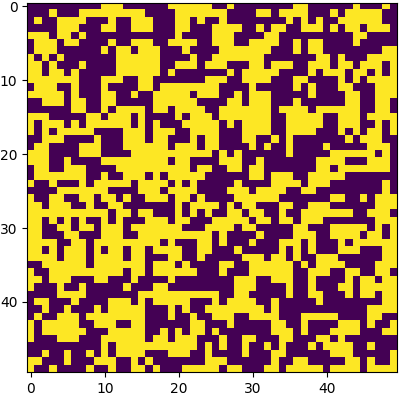
\includegraphics[width=0.95\textwidth]{images/ising-glauber-high-temp-result}
            \caption[The result of running Glauber dynamics at a high temperature.]{The result of running Glauber dynamics at a high temperature. Here a \enquote{high temperature} is \(T = 5\) in units where \(\boltzmann = J = 1\). Notice that the pattern of spins appears fairly random but there are slightly more yellow sites than purple.}
        \end{subfigure}
        \hspace{1em}
        \begin{subfigure}[t]{0.45\textwidth}
            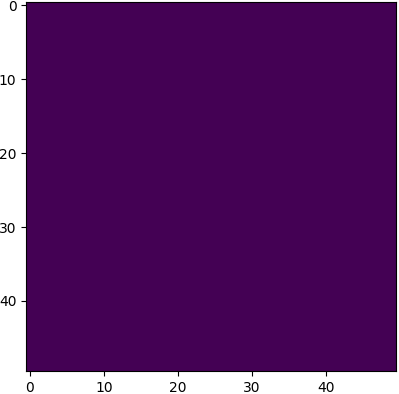
\includegraphics[width=0.95\textwidth]{images/ising-glauber-low-temp-result}
            \caption[The result of running Glauber dynamics at a low temperature.]{The result of running Glauber dynamics at a low temperature. Here a \enquote{low temperature} is \(T = 0.01\) in units where \(\boltzmann = J = 1\).}
        \end{subfigure}
        \begin{subfigure}[t]{0.45\textwidth}
            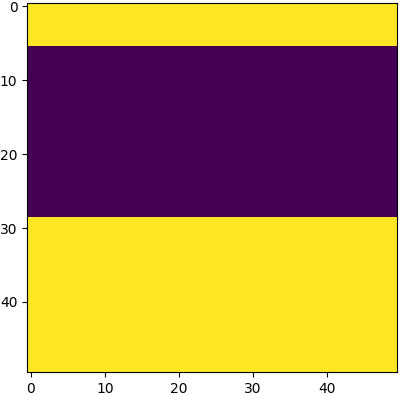
\includegraphics[width=0.95\textwidth]{images/ising-glauber-metastable}
            \caption[Metastable state]{A metastable state in the Glauber dynamics. The boundary being straight lines minimises the number of neighbouring unaligned spins. This state will remain for a long time but eventually all spins will align.}
        \end{subfigure}
        \hspace{1em}
        \begin{subfigure}[t]{0.45\textwidth}
            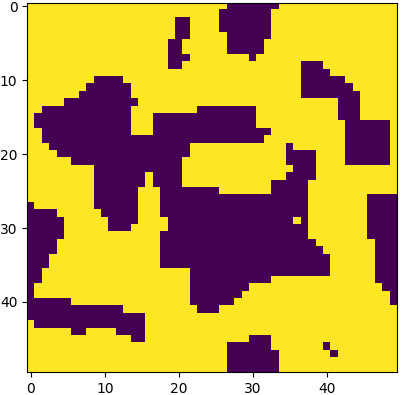
\includegraphics[width=0.95\textwidth]{images/ising-glauber-low-temp-part-way}
            \caption[A few steps into Glauber dynamics.]{The result of 10 sweeps with low temperature Glauber dynamics. One sweep meaning attempting to change \(N\) spins, where \(N\) is the total number of spins (here \(N = 2500\). Even after a relatively short time the spins separate into domains.}
        \end{subfigure}
        \caption{Various results of running Glauber dynamics for \(N = 50^2 = 2500\) spins.}
    \end{figure}
    
    \section{Kawasaki Dynamics}
    In Glauber dynamics we often end up with all spins aligned.
    This isn't always reasonable.
    Sometimes the net \defineindex{magnetisation} of a system,
    \begin{equation}
        M \coloneqq \sum_{i=1}^{N} S_i,
    \end{equation}
    is fixed.
    One way to model this sort of system is with Kawasaki dynamics.
    
    In Kawasaki dynamics we generate the next state by choosing two random spins and then swapping them.
    We now consider only what happens if the chosen spins are different since if their the same nothing changes.
    If these spins \emph{aren't} nearest neighbours then the change in energy is simply
    \begin{equation}
        \Delta E = 2JS_i \sum_{\langle i, k \rangle} S_k + 2JS_j \sum_{\langle j, l \rangle} S_l
    \end{equation}
    where \(i\) and \(j\) are the indices of the spins we swap.
    The logic for this is that this is essentially the same as repeating the Glauber dynamics process twice with these two spins chosen.
    
    If the spins are nearest neighbours then we have to be more careful calculating the energy change but it can still be done in an \(\order(1)\) way by carefully considering which spins are actually effected by the swap.
    
    Since we are only swapping spins the net magnetisation remains the same.
    This means that the results tend to have spins group into domains where they are all aligned since this minimises the energy.
    Of course if the temperature is high enough then entropy dominates and we get essentially random states indistinguishable from Glauber dynamics.
    
    % TODO: Add picture from Kawasaki dynamics
    
    \section{Measurements}
    Once we have a simulation running one of these dynamical algorithms we want to make measurements of the system.
    One of our goals will be to find the \defineindex{critical temperature}, \(T_{\mathrm{c}}\), which is the temperature at which the system goes from ordered to random.
    This is the temperature which distinguishes the \enquote{low temperature} cases from the \enquote{high temperature} cases.
    
    Two observables which we have already mentioned are the energy,
    \begin{equation}
        E = -J\sum_{\langle i, j \rangle} S_iS_j,
    \end{equation}
    and magnetisation,
    \begin{equation}
        M = \sum_{i=1}^{N} S_i.
    \end{equation}
    We expect that the energy will be much lower for an ordered phase and much higher for a disordered phase since spins align more in the ordered phase.
    For Glauber dynamics the magnetisation will tend to \(\pm N\) for low temperatures as all spins align.
    For this reason we consider the absolute value of the magnetisation, since there is nor real logic to assigning one spin as \(+1\) and the other as \(-1\) so the sign cannot have physical meaning.
    For Kawasaki dynamics \(M\) is constant so not that useful.
    
    The average energy is given by the Monte Carlo approximation as
    \begin{equation}
        \expected{E} = \frac{1}{n} \sum_{i=1}^{n} E(\mu_i)
    \end{equation}
    where \(\{\mu_i\}\) are all states visited and \(E(\mu_i)\) is the energy in state \(\mu_i\), and \(n\) is the total number of states visited, we take \(n\) to be large for this to be a good approximation.
    Similarly the average absolute magnetisation is
    \begin{equation}
        \expected{\abs{M}} = \frac{1}{n} \sum_{i=1}^{n} \abs{M(\mu_i)}
    \end{equation}
    where \(M(\mu_i)\) is the magnetisation in state \(\mu_i\).
    
    Consider what happens in Glauber dynamics.
    At a low temperature we expect that the spins align and so \(\expected{E} = -2JN\), since either \(S_i\) and \(S_j\) are both \(+1\) or both \(-1\), either way their product is \(+1\) and so we eventually achieve constant (up to random fluctuations of a few spins) energy \(-2JN\) and over enough time the states that occurred before achieving this have negligible impact on the average.
    At high temperatures the spins are essentially random so \(S_i\) and \(S_j\) are just as likely to have the same sign as the opposite sign and hence in the energy sum most terms cancel out and we get \(\expected{E} = 0\), again, up to random fluctuations.
    
    The case of magnetisation is similar with \(\expected{\abs{M}} = N\) at low temperatures and \(\expected{\abs{M}} = 0\) at high temperatures.
    
    % TODO: add images of plots showing results
    
    How can we use this to find the critical temperature?
    First we consider what happens when the number of spins, \(N\), tends to infinity.
    In this case we get two very clear regions of low and high temperature.
    This is shown in \cref{fig:averages for infinite spins}.
    Notice the discontinuity at the critical temperature, \(T_{\mathrm{c}}\).
    For small \(N\) however this discontinuity can't be seen.
    
    \begin{figure}
        \begin{tikzpicture}
            \draw[<->, very thick] (0, 4) node[above] {\(\expected{\abs{M}}\)} -- (0, 0) -- (4.2, 0) node[right] {\(T\)};
            \draw[ultra thick, highlight] (0, 3) -- ++ (2, 0) -- ++ (0, -3) -- ++ (2, 0);
            \node[below] at (2, 0) {\(T_{\mathrm{c}}\)};
            \begin{scope}[xshift=5cm]
                \draw[<-, very thick] (0, 4) node[above] {\(\expected{E}\)} -- (0, 0);
                \draw[->, very thick] (0, 3) -- (4.2, 3) node[right] {\(T\)};
                \draw[ultra thick, highlight] (0, 0.5) -- ++ (2, 0) -- ++ (0, 2.5) -- ++ (2, 0);
                \node[above] at (2, 3) {\(T_{\mathrm{c}}\)};
            \end{scope}
        \end{tikzpicture}
        \caption[Average absolute magnetisation and energy for an infinite number of spins.]{Plots of the average absolute magnetisation and energy for an infinite number of spins. Notice the sudden change at the critical temperature, \(T_{\mathrm{c}}\).}
        \label{fig:averages for infinite spins}
    \end{figure}
    
    Instead of the discontinuity we use the fact that fluctuations tend to be very large near the critical temperature as the system moves back and forth between the two phases.
    One measure of the fluctuations is the standard deviation,
    \begin{equation}
        \sigma_E \coloneqq \expected{E^2} - \expected{E}^2.
    \end{equation}
    However, by dividing by \(N\boltzmann T^2\) we can associate this with the specific heat capacity, \(C\), per spin:
    \begin{equation}
        \frac{\expected{E^2} - \expected{E}^2}{N\boltzmann T^2} = \frac{C}{N}.
    \end{equation}
    Similarly for the magnetisation we can relate the standard deviation to the susceptibility, \(\chi\), per spin:
    \begin{equation}
        \frac{\expected{M^2} - \expected{M}^2}{N\boltzmann T} = \frac{\chi}{N}.
    \end{equation}
    
    Plotting these quantities will give a peak at \(T_{\mathrm{c}}\).
    The height of the peak will vary with \(\ln N\) whereas away from the peak the values will be approximately constant with respect to \(N\).
    
    % TODO: Add plots of C/N and χ/N
    
%    %   Appdendix
%    \appendixpage
%    \begin{appendices}
%        \include{}
%    \end{appendices}

\backmatter
\renewcommand{\glossaryname}{Acronyms}
\printglossary[acronym]
\printindex
\end{document}